% Latex template: https://github.com/mqTeXUsers/Macquarie-University-Beamer-Theme

% Slide Masters:

% Title
% Text
% 2 column
% Full-image
% Bibliography
% Closing
 
\documentclass[aspectratio=169, 12pt]{beamer} % Aspect ratio
% https://tex.stackexchange.com/a/14339/5483 
% Possible values: 1610, 169, 149, 54, 43 and 32.
% 169 = 16:9

\PassOptionsToPackage{table}{xcolor}    %https://tex.stackexchange.com/a/5365/5483

\usetheme{macquarie}
\usepackage{multicol} % https://tex.stackexchange.com/a/396018/5483

\usepackage{svg} %https://github.com/mrpiggi/svg 

\usepackage[english]{babel}       % Set language
% \usepackage[utf8x]{inputenc}      % Set encoding
\usepackage{colortbl}
\mode<presentation>           % Set options
{
  \usetheme{default}          % Set theme
  \usecolortheme{default}         % Set colors
  \usefonttheme{default}          % Set font theme
  \setbeamertemplate{caption}[numbered] % Set caption to be numbered
}

% Uncomment this to have the outline at the beginning of each section highlighted.
%\AtBeginSection[]
%{
%  \begin{frame}{Outline}
%    \tableofcontents[currentsection]
%  \end{frame}
%}

\usepackage{graphicx}         % For including figures
\usepackage{booktabs}         % For table rules
\usepackage{hyperref}         % For cross-referencing

\usepackage{enumitem} % https://tex.stackexchange.com/a/2292/5483

\usepackage{comment}

%https://tex.stackexchange.com/a/371844/5483
\setbeamerfont{bibliography entry author}{size=\tiny}
\setbeamerfont{bibliography entry title}{size=\tiny}
\setbeamerfont{bibliography entry location}{size=\tiny}
\setbeamerfont{bibliography entry note}{size=\tiny}
\setbeamerfont{bibliography item}{size=\tiny}

%https://tex.stackexchange.com/q/333587/5483

\title{FAIMS 3.0: Electronic Field Notebooks} % Presentation title
\author{SA Ross, B Ballsun-Stanton, S Cassidy, P Crook, A Sobotkova, J Klump}   % Presentation author
\institute{CAA Australasia Online Conference}   % Author affiliation
\date{11 September 2020}    % Presentation date  


\begin{document}

% Title page
% This page includes the informations defined earlier including title, author/s, affiliation/s and the date
% \begin{frame}[noframenumbering]

\maketitle

 
% \end{frame}


% Outline
% This page includes the outline (Table of content) of the presentation. All sections and subsections will appear in the outline by default.
\begin{frame}{Strategies for field data capture infrastructure}
  \tableofcontents
\end{frame}

% The following is the most frequently used slide types in beamer
% The slide structure is as follows:
%
%\begin{frame}{<slide-title>}
% <content>
%\end{frame}

% Slides to speak to at CAA2019

% In-depth information for reference

\section{`Small data' infrastructure}

\begin{frame}{`Small data' research}
 \begin{figure}[H]
    \centering
        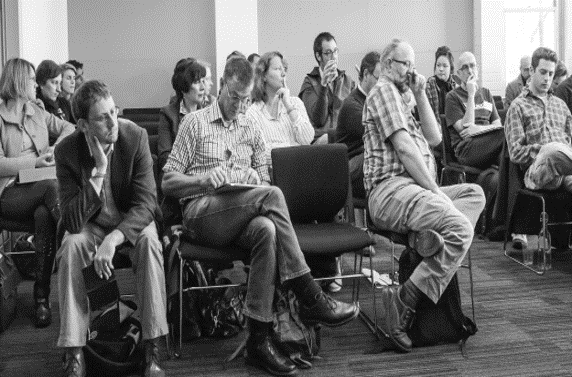
\includegraphics[height=.75\textheight]{figures/Archaeologists-standards.png}
        \caption{Archaeologists contemplate data standards (FAIMS Stocktaking, 2012)}
        \label{fig:figure7}
 \end{figure}
\end{frame}

% \begin{frame}{Context: the challenge of `small data'}
%     `Long tail' research: most field data is small data \cite{Borgman2015-rh}
%     \begin{itemize}[label=\textbullet]
%         \item Smaller scale; smaller communities; local control.
%         \item Diverse questions, approaches, and methods.
%         \item Heterogeneous data; variety of content, structure.
%         \item Data and infrastructure emerge from fieldwork. 
%         \item Relative lack of standards.
%         \item Limited infrastructure and funding.
%         \item Challenges associated with big(ger) data from photogrammetry, SfM, video, geophysics, etc., will exacerbate these problems.
%     \end{itemize}
% \end{frame}

% Brian's suggestion
\begin{frame}{Context: the challenge of `small data'}
    `Long tail' research: most field data is small data \cite{Borgman2015-rh}
    \begin{itemize}[label=\textbullet]
        \item Smaller scale
        \item Diverse approaches
        \item Heterogeneous data
        \item Data and infrastructure emerge from fieldwork. 
        \item Relative lack of standards.
        \item Limited funding.
        \item Large(r) new data streams make everything worse.
        % \item Challenges associated with big(ger) data from photogrammetry, SfM, video, geophysics, etc., will exacerbate these problems.
    \end{itemize}
\end{frame}



\begin{frame}{The data lifecycle}
 \begin{figure}[H]
    \centering
        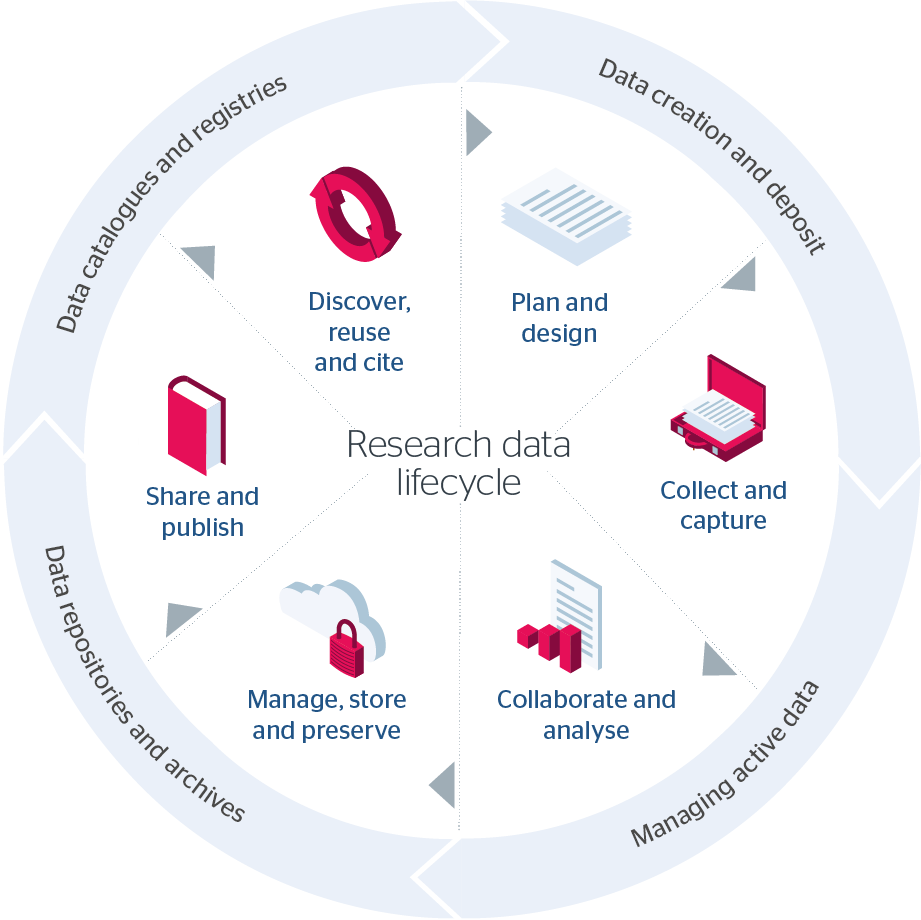
\includegraphics[height=.75\textheight]{figures/research-data-life-diagram.png}
        \caption{\cite{Jisc2018-gx} Image CC-BY-ND}
        \label{fig:figure9}
 \end{figure}
\end{frame}

\begin{frame}{Infrastructure across the data lifecycle}
    Three main phases of the data lifecycle
    \begin{itemize}[label=\textbullet]
        \item Publication (most mature)
        \item Processing and analysis (less mature ) \cite{Stewart_Lowndes2017-lj} \cite{Alveo2019-tk}.
        \item Capture (least mature and least supported by `normal' tools) \cite{Bureau_of_Reclamation2017-xl}.
    \end{itemize}
\end{frame}


\section{Eight years of FAIMS Mobile}

\begin{frame}{Research Specific}
 \begin{figure}[H]
    \centering
        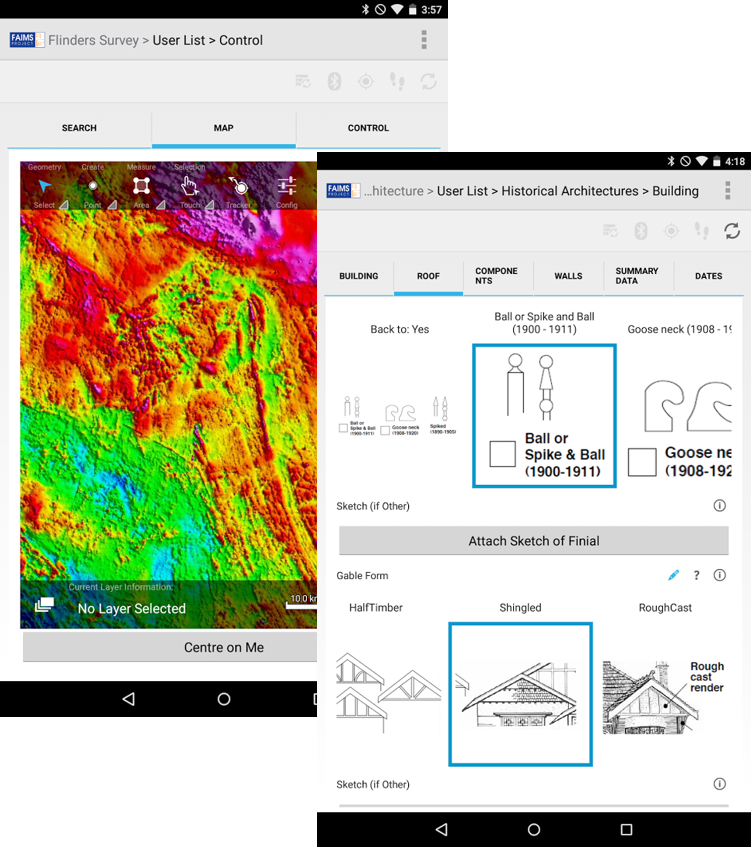
\includegraphics[height=.75\textheight]{figures/FAIMS-screenshots.png}
        \caption{FAIMS Mobile: GIS and `picture dictionaries'}
        \label{fig:FAIMS-mobile-screenshots}
 \end{figure}
\end{frame}


%\begin{frame}[allowframebreaks]{Key research-specific features}
\begin{frame}{Key research-specific features}
\begin{multicols}{2}
\begin{itemize}[label=\textbullet]
        \item Customisable workflows.
        \item Offline capable.
        \item Complete data provenance / version history.
        \item Binds text, structured, geospatial, multimedia data.
        \item Mobile GIS with layers, raster and vector display, shape creation.
        \item Uses device and external sensors. 
        \item Multimedia file and metadata management.
        \item Validation and automation on device or server.
        \item Multilingual user-interface.
        \item Granular metadata: Notes and certainty for each field.
        \item Contextual help with images.
        \item Structured data can implement vocabularies / ontologies, LOD approaches.
        \item Data can be exported in a variety of formats, including custom exports.
    \end{itemize}
\end{multicols}
    
\end{frame}

\begin{frame}{Generalised}
 \begin{figure}[H]
    \centering
        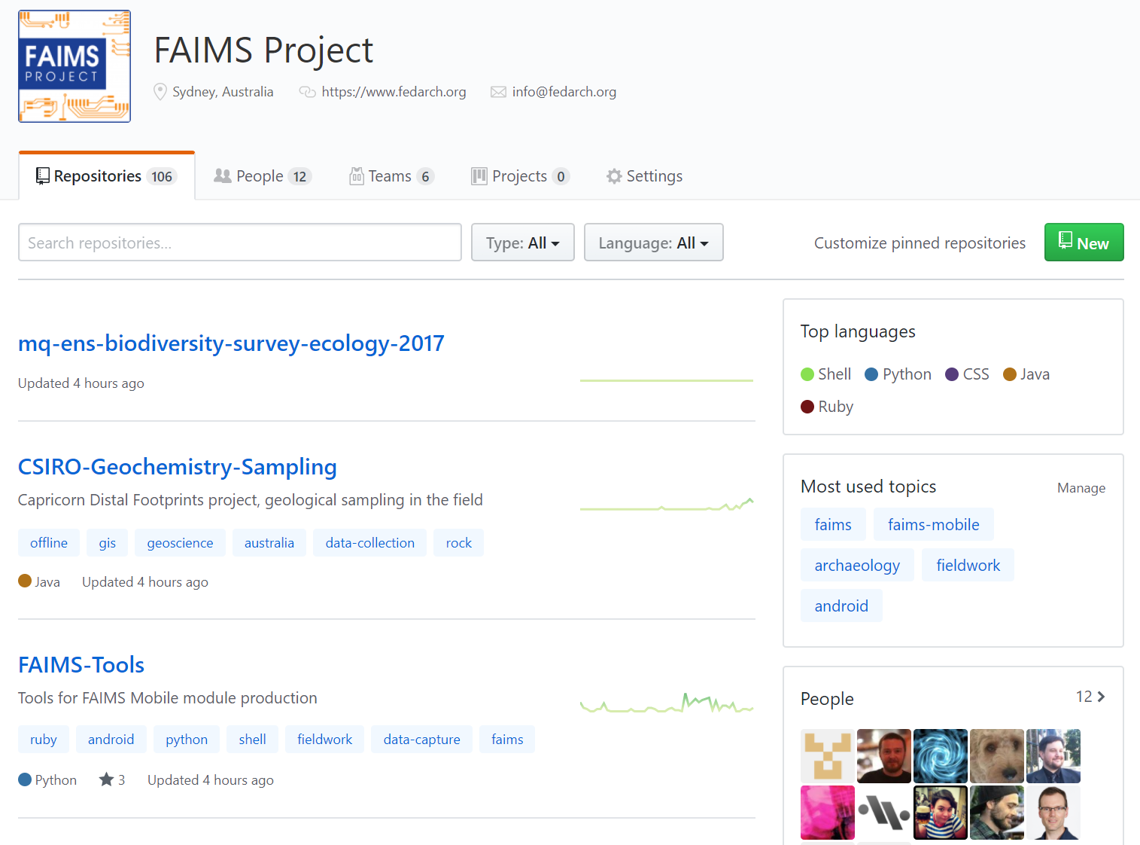
\includegraphics[height=.75\textheight]{figures/FAIMS-generalised.png}
        \caption{FAIMS Mobile customisations on GitHub}
        \label{fig:FAIMS-github}
 \end{figure}
\end{frame}

\begin{frame}{Modular and federated}
 \begin{figure}[H]
    \centering
        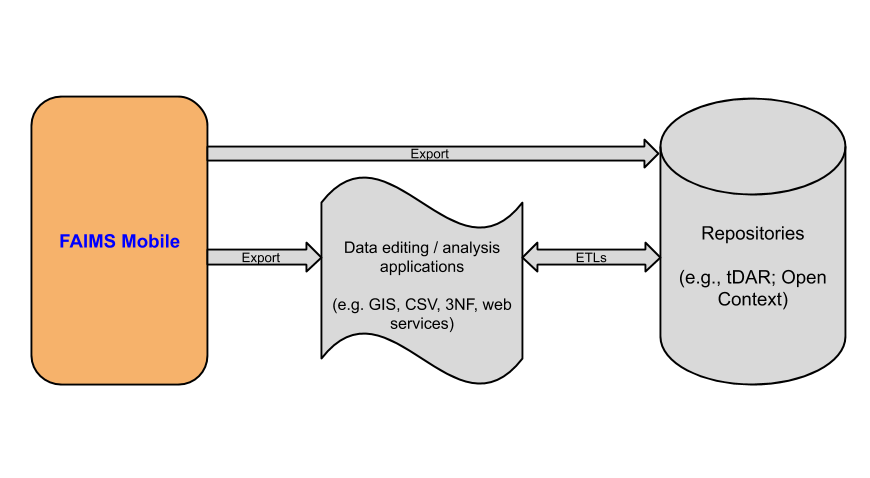
\includegraphics[height=.75\textheight]{figures/FAIMS-federation}
        \caption{FAIMS Mobile federation}
        \label{fig:FAIMS-federation}
 \end{figure}
\end{frame}

\begin{frame}{Open Source}
 \begin{figure}[H]
    \centering
        
\includegraphics[width=.75\textwidth]{figures/GPLv3_Logo.eps}
        \caption{FAIMS Mobile `core' code is GPLv3; definition files are openly licensed; everything is on GitHub}
        \label{fig:FAIMS-github-OSS}
 \end{figure}
\end{frame}


\begin{frame}{FAIMS by the numbers}
 \begin{itemize}[label=\textbullet]
        \item \textbf{63 field data capture workflows customised}.
        \item \textbf{47 workflows confirmed deployed} to field at over \textbf{40 projects}.
        \item \textbf{100s of users} logged \textbf{10,000s hours} on the platform.
        \item Deployments took place in disciplines including \textbf{archaeology, geoscience, ecology, oral history, ecology, }and \textbf{linguistics}.
    \end{itemize}
\end{frame}

\begin{frame}{Example deployments}
 \begin{itemize}[label=\textbullet]
        \item Indigenous Foodways in the Cape York Peninsula (UNE, archaeology)
        \item Khirbet el-Rai Excavations, Israel (Macquarie, archaeology).
        \item Landscape Archaeology at Lake Mungo (LTU, archaeology)
        \item Excavation at the Boncuklu Höyük, Turkey (UQ, archaeology).
        \item Tao River Archaeological Project, China (Harvard, archaeology).
        \item Proyecto Arqueològico Zaña Colonial, Peru (Brown, archaeology).
        \item The Malawi Earlier-Middle Stone Age Project (Yale, archaeology).
        \item Avian Ecology in NSW (Macquarie, ecology)
        \item The Greek-Australian Historical Archive (UNSW, oral history).
        \item Key Pluridisciplinary Advances on African Multilingualism, Cameroon (SUNY Buffalo, linguistics).
        \item Capricorn Distal Footprints Project (CSIRO, geological sampling).

    \end{itemize}
\end{frame}

\section{FAIMS 3.0}

\begin{frame}{Where are we now?}
    \begin{itemize}[label=\textbullet]
        \item FAIMS v2.6 is nearing end of its useful life.
        \item The FAIMS team did CSIRO ON Prime in 2016, completing 70+ interviews with clients / potential clients.
        \item A high-level technical plan for FAIMS v3.0 won a US design prize in 2017 \cite{Bureau_of_Reclamation2017-xl}.
        \item ARDC Platforms grant awarded in late 2019 to rebuild FAIMS using modern components.
    \end{itemize}
\end{frame}

\begin{frame}{Opportunities and challenges}
    \begin{itemize}[label=\textbullet]
        \item Useful research-specific features of FAIMS v2.6 to be retained.
        \item Android-only hindered uptake; cross-platform support required.
        \item Lack of self-service customisation / deployment hindered uptake.
        \item Users want to be able to edit data on the desktop or online, then have that data available for further editing in the field (data `round-trip' outside of the application).
        \item Users want more options for accessing / exporting data on-demand.
        \item Users want to be able to use the platform for sensitive data. 
        \item Improved scalability needed (application performance; server-to-server synchronisation)
        \item Enterprise features (orchestration, user management, reporting, branding, SSO, etc.) needed for eventual COSS \textbf{product} to support sustainability (underlying software \textbf{project} will remain OS).
    \end{itemize}
\end{frame}

\begin{frame}{Approaches under consideration}
Technical elaboration has now begun (September 2020); technology candidates include:
    \begin{itemize}[label=\textbullet]
        \item Cross-platform frameworks (e.g., Flutter, Cordova)
        \item NoSQL datastores (e.g., Apache CouchDB / PouchDB).
        \item Javascript map tilers (e.g., Leaflet).
        \item Definition files in JSON rather than XML.
        \item API development. 
        \item Web application to provide GUI to produce definition files.
        \item 'Real' user management and security.
        \item Interoperability with Cloudstor, VLs / Gateways, domain repositories.
    \end{itemize}
\end{frame}

\begin{frame}{Thank you!}
PDF and source code for this presentation is available at: 
\texttt{https://github.com/saross/FAIMS-intro/releases/tag/v3.0}.

FAIMS 3.0 project website: \texttt{https://osf.io/mqk45/}.

FAIMS Project software, customisation library, and documentation can be found at:
\texttt{https://github.com/faims}.


This work is licensed under a Creative Commons Attribution 4.0 International License.

\end{frame}


\section{References}

% Adding the option 'allowframebreaks' allows the contents of the slide to be expanded in more than one slide.
% The "1" comes from the outer theme"

% \begin{frame}[allowframebreaks]{References}
  
%   \bibliography{references}
%   \bibliographystyle{apalike}
% \end{frame}

\begin{multicols}{2}[]
\bibliographystyle{apalike}

\bibliography{references}
\end{multicols}


% In-depth information or additional details for reference

\section{Extras: CAA Australasia Abstract}

\begin{frame}[allowframebreaks]{Abstract}
    
    Fieldwork is time consuming and researchers are always looking at ways to increase efficiency in data recording in the field, while also improving our ability to share reusable data following international good practices like the Transparency and Openness Principles (TOP) and Findable, Accessible, Interoperable, and Reusable (FAIR) data principles. Achieving these goals is easier when data is born digital, but commercial software is not optimised for research and bespoke software is expensive to build and onerous to maintain. The Australian Research Data Commons (ARDC) recently awarded the Field Acquired Information Management Systems (FAIMS) Project, based at Macquarie University, a large, three-year grant to renew our existing platform, FAIMS Mobile, which has been customised and deployed at more than 60 workflows on 40 projects worldwide but is reaching end-of-life. FAIMS Electronic Field Notebooks will produce and manage mobile apps for a range of disciplines including not only archaeology, but earth sciences, ecology, and oral history, ensuring data is captured consistently and is well documented. The platform will use modern web technologies and integrate with existing analysis environments to provide a seamless workflow. FAIMS Electronic Field Notebooks will accommodate diverse data capture, localisation and complex workflows, and provide seamless synchronisation, backup and version control, just like FAIMS Mobile. It will also be cross-platform (Android, iOS and Desktop) and self-service allowing uses to customise and deploy modules through a graphic user interface. This presentation will introduce the next generation of FAIMS, and how it can contribute to open research in archaeology.
    
    * * *
    
    Session 3: Data Management, \href{https://au.caa-international.org/online-conference-2020/}{CAA Australasia Online Conference, 11-12 September 2020} 
    
    \emph{Delivered Friday 11 September by Shawn A Ross}
    
\end{frame}

\section{Extras: FAIMS research-specific features}

\begin{frame}[allowframebreaks]{Key research-specific features}
    \begin{itemize}[label=\textbullet]
        \item Workflows and data schemata are deeply customisable.
        \item Customisation is achieved using relatively simple and human-readable XML documents separate from the ‘core’ software, supporting sharing, modification, and reuse via collaborative software development platforms like GitHub.
        \item Resulting mobile applications work offline.
        \item Automated bi-directional synchronisation using local or online server.
        \item A complete version history, with review and selective rollback, is provided for all data.
        \item Binds structured, geospatial, multimedia, and free text data in one record.
        \item A mobile GIS provides layer management and tools for the creation and editing of shapes.
        \item Connects to internal and external sensors (e.g., Bluetooth / USB devices).
        \item Externally captured multimedia (e.g., dSLR photos, audio recordings) can be connected to a record, then data contained in the associated record can be used to automatically rename connected multimedia files or write file metadata.
        \item Data validated on device and/or on server.
        \item Applications can be made multilingual using a standard and well-established localisation approach..
        \item Granular and contextualised metadata and certainty.
        \item Granular and contextualised help, including images, can be provided for all data entry fields.
        \item All data entry fields can be mapped to shared vocabularies, thesauri, or ontologies via embedded URIs, supporting Linked Open Data approaches.
        \item Data can be exported from the server in a variety of formats, or can be customised to a specific data target (e.g., JSON, relational database).
    \end{itemize}
\end{frame}

\section{Extras: The FAIMS approach in-depth}

\begin{frame}{Introduction to the FAIMS Project}
    \begin{itemize}[label=\textbullet]
        \item The Field Acquired Information Management Systems (FAIMS) Project began in 2012 as a national Australian information infrastructure project in archaeology.
        \item Developed FAIMS Mobile for field data capture \cite{Ballsun-Stanton2018-zd}.
        \item Use expanded beyond archaeology to geoscience, ecology, ethnography, linguistics, oral history.
        \item Has been customised for over 50 workflows at more than 30 projects. 
        \item Data and workflow modelling for customisations provided deep insights into field data capture and the infrastructure needed to support it.
    \end{itemize}
\end{frame}

\begin{frame}{FAIMS Mobile software}
 \begin{figure}[H]
    \centering
        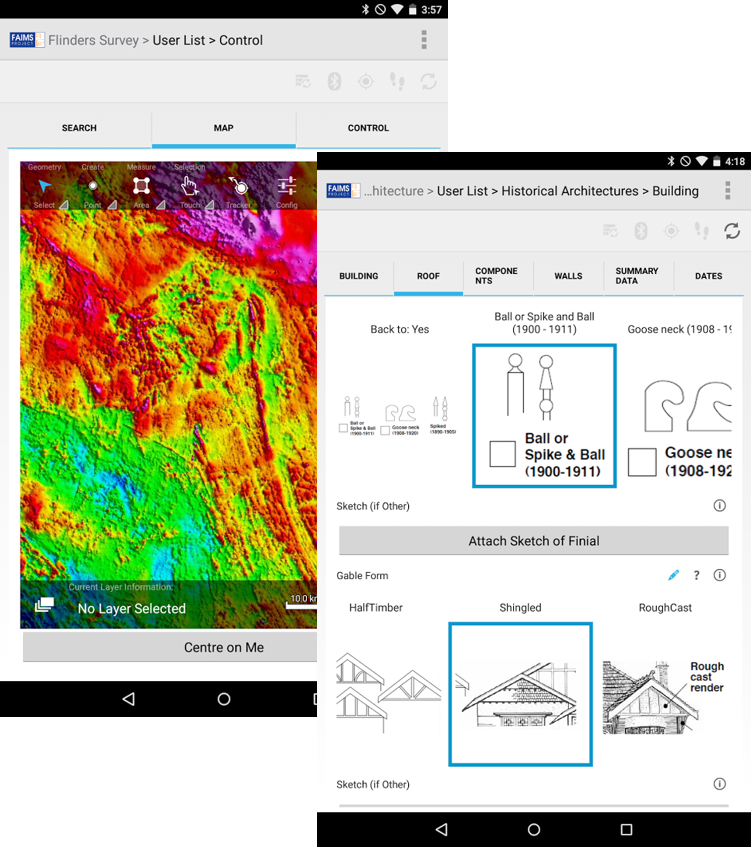
\includegraphics[height=.75\textheight]{figures/FAIMS-screenshots.png}
        \caption{FAIMS Mobile: GIS and `picture dictionaries'}
        \label{fig:figure10}
 \end{figure}
\end{frame}

\begin{frame}{Field data capture infrastructure: a manifesto}
    \begin{itemize}[label=\textbullet]
        \item Our domains deserve research-specific software.
        \item Diverse practices and limited resources require generalised software.
        \item Do one thing well with modular and federated software (but slice the pie thoughtfully).
        \item Open-source software supports open research and has other advantages (but is difficult to sustain). 
        \item Scope requirements carefully.
        \item Invest in outreach and engagement.
    \end{itemize}
\end{frame}

\begin{frame}{Research specific}
    Field research needs (and deserves) research-specific software, contra \cite{Roosevelt2015-kd}.
      \begin{itemize}[label=\textbullet]
        \item Most commercial / mass-market software does not meet research needs.
        \item Risk of lock-in, unwelcome changes to features or business models, and product discontinuation.
    \end{itemize}
    Compare ecology: TERN, ALA, Biocollect, and associated research clouds \cite{Tern2019-sp, Ala2019-by, Ala2019-cb}.
\end{frame}

\begin{frame}{Generalised (not generic or bespoke)}
  Commercial software doesn't meet our needs, and bespoke development is too expensive and usually unsustainable.
      \begin{itemize}[label=\textbullet]
        \item Generalised software can be deeply customised to accommodate our diverse data types, data models, workflows, etc.
        \item The code used to customise it describes the data model and workflow.
        \item Customisations can be published and re-deployed trivially.
        \item Can deliver research-grade software affordably.  
    \end{itemize}
    FAIMS Mobile cost perhaps 3x a single bespoke application, but has been customised 50x. Customisation cost is 1/10th bespoke, and still <1/2 even if `core' platform development costs are amortised across projects.
\end{frame}

\begin{frame}{Generalised: customise using code}
 \begin{figure}[H]
    \centering
        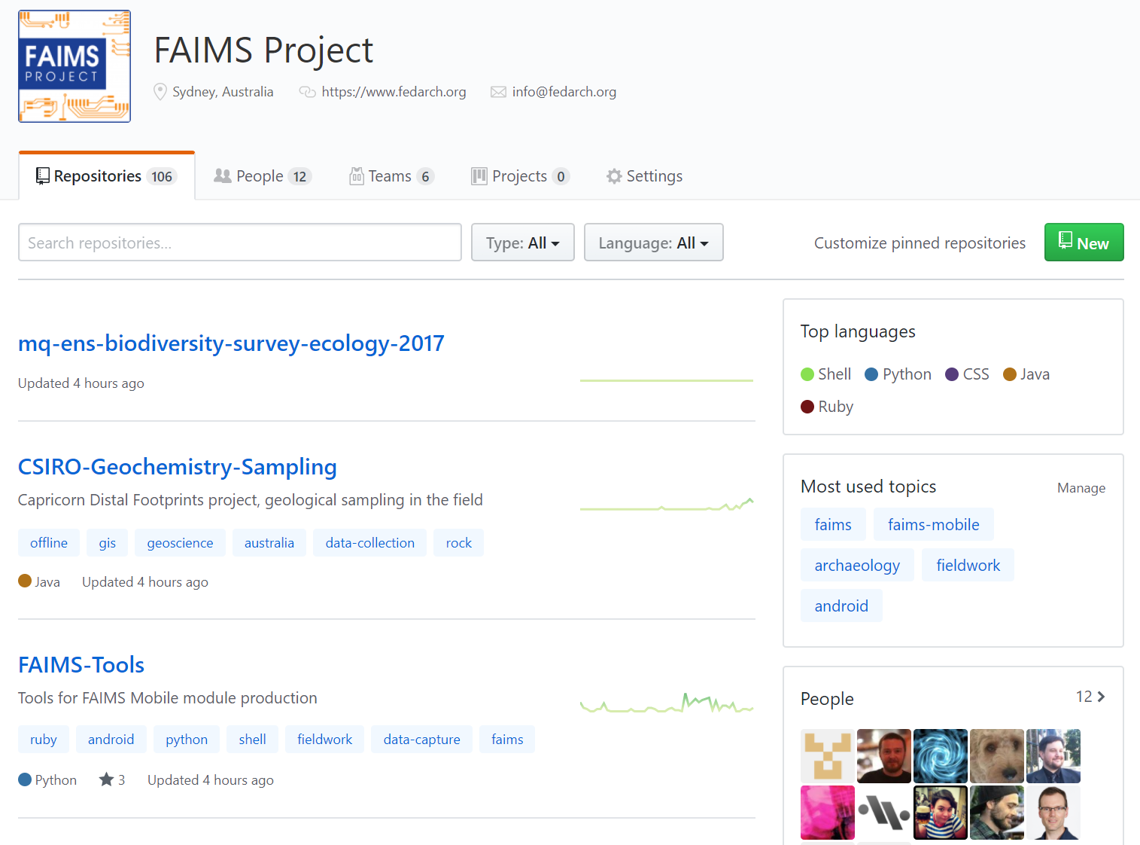
\includegraphics[height=.75\textheight]{figures/FAIMS-generalised.png}
        \caption{FAIMS Mobile customisations (XML files, mostly) on GitHub}
        \label{fig:figure11}
 \end{figure}
\end{frame}

\begin{frame}{Modular and federated}
  Do one thing well.
      \begin{itemize}[label=\textbullet]
        \item Identify other infrastructure in the domain and interoperate with it (via ETLs or APIs).
        \item It is better to divide by data-lifecycle phase rather than data type, since (1) our data is so integrated and (2) field data capture poses unique challenges.
    \end{itemize}
\end{frame}

\begin{frame}{Modularise by data lifecycle phase}
 \begin{figure}[H]
    \centering
        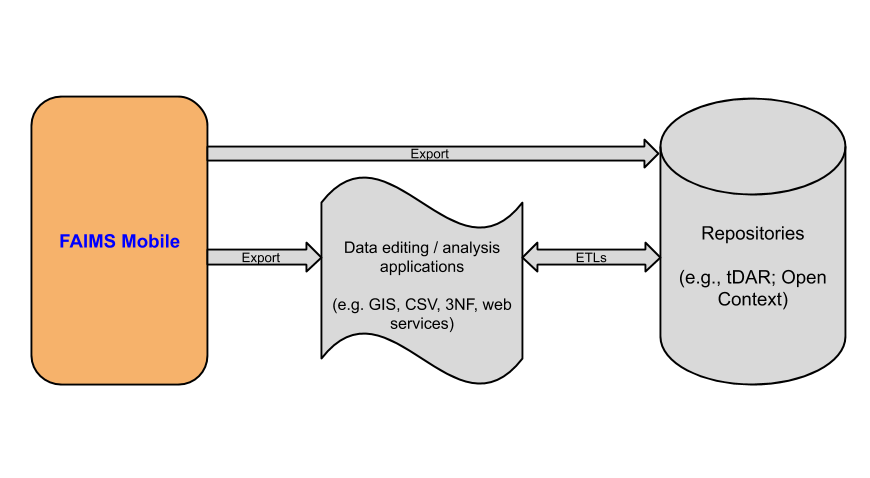
\includegraphics[height=.75\textheight]{figures/FAIMS-federation.png}
        \caption{FAIMS Mobile federation strategy}
        \label{fig:figure13}
 \end{figure}
\end{frame}

\begin{frame}{Open source?}
  Open source has advantages but is difficult to sustain.
      \begin{itemize}[label=\textbullet]
        \item Emerging open research principles strongly prefer OSS as opposed to proprietary ‘black boxes’.
        \item Transparency and reusability (esp. customisation code).
        \item Ability to hand off from one organisation to another (esp. `core' platform code).
        \item Ability to fork code prevents lock-in and mitigates unwelcome decisions by software developers.
        \item BUT OSS business models are hard to scale and rely on occasional injections of grant or institutional funding.
    \end{itemize}
\end{frame}

\begin{frame}{Scope carefully}
  Talk to a wide range of potential users, seeking facts not opinions.
      \begin{itemize}[label=\textbullet]
        \item Don’t ask researchers what they think, ask them what they have done - what software they have adopted and why, and what problems they have expended resources to solve. 
        \item ‘Lean startup’ methodology very useful, based around  testing of ideas through interviews with potential users \cite{Strategyzer_AG2019-uu}.
        \item In our case, we over-invested in mobile GIS and under-invested in usability (especially a GUI for customisation).
    \end{itemize}
\end{frame}

\begin{frame}{Spend on outreach and engagement}
  If you build it they will not come; people can't use technologies they don't know about.
      \begin{itemize}[label=\textbullet]
        \item As per industry standards, dedicate at least 30\% of any information infrastructure budget to outreach and engagement (sales and marketing). 
        \item Typical academic outreach (journal articles, conference presentations, workshops, even booths at major conferences) are not enough.
    \end{itemize}
\end{frame}

\section{Extras: Reports from the field}

\begin{frame}[allowframebreaks]{User feedback}
    \begin{itemize}[label=\textbullet]
        \item ``The tablet app worked very well in the field and I would be keen to continue using it for subsequent sampling'' -- New Zealand Soil Geochemistry
        \item ``Being able to check in on everyone's work from my computer so easily is... revolutionary. Thank you for building such an amazing tool! …  I look forward to providing more details, but I already feel like I have 100\%{} better control over data quality, even compared to last year'' -- Proyecto Arquelogico de Zana Colonial
        \item ``The app has been such an incredible advantage in terms of workload, data quality, and a number of other data management issues with which archaeologists regularly have to deal. It readily links disparate data types that are otherwise stored separately – such as photographs, tabular logs, and context relationships.'' -- Malawi Early-Middle Stone Age Project
        \item ``I was really impressed with the approach FAIMS project has taken to the challenge of creating field data apps which can be very expensive. Our module was ready for testing after just one briefing.'' -- Streamwatch
        \item ``We’re back from the field and I cannot believe how well everything went. ... [T]he combination of the mobile lab, the sample ID/tracking and FAIMS application enabled us to average 5-6 minutes per sample site (crust, soil, rock and two plants)  in the field and about half that in the lab... Using the old school notepad and GPS approach this would have been 15 mins at best and a whole lot of misplaced photos and details, not to mention the additional hours entering the data in at night. We were able to identify missed sites as we went and completed the soils map (280 sites) and infill (36 sites) and analysis all in the 7 days. '' -- CSIRO Mineral Resources
    \end{itemize}
\end{frame}

\section{Extras: FAIMS publications}

\begin{frame}[allowframebreaks]{FAIMS publications}
\small{ \url{https://www.zotero.org/groups/2542876/faims-project/library}

        \nocite{Ross2020-yg,Noble2019-qg,Ballsun-Stanton2018-zd,Sobotkova2018-al,VanValkenburgh2018-hv,Sobotkova2016-mx,Ross2015-ph,Sobotkova2015-lq,Ross2013-hi}
        
        Ross, S. A., \& Ballsun-Stanton, B. (Accepted 02 April 2020). Introducing Preregistration of Research Design to Archaeology. In E. Watrall \& L. Goldstein (Eds.), Digital Heritage and Archaeology in Practice. University Press of Florida.
        
        Noble, R., Gonzalez-Alvarez, I., Reid, N., Krapf, C., Pinchand, T., Fox, D., Ibrahimi, T., Cole, D., \& Lau, I. (2019). Coompana geochemistry - results from rapid surface characterization and a deep vertical profile. South Australia MESA Journal, 89, 4–14. http://hdl.handle.net/102.100.100/86035?index=1
        
        Ballsun-Stanton, B., Ross, S. A., Sobotkova, A., \& Crook, P. (2018). FAIMS Mobile: Flexible, open-source software for field research. SoftwareX, 7C, 47–52. https://doi.org/10.1016/j.softx.2017.12.006
        
        Sobotkova, A. (2018). Sociotechnical Obstacles to Archaeological Data Reuse. Advances in Archaeological Practice, 6(2), 117–124. https://doi.org/10.1017/aap.2017.37
        
        VanValkenburgh, P., Silva, L. O. G., Repetti-Ludlow, C., Gardner, J., Crook, J., \& Ballsun-Stanton, B. (2018). Mobilization as Mediation: Implementing a Tablet-Based Recording System for Ceramic Classification. Advances in Archaeological Practice, 1–15. https://doi.org/10.1017/aap.2018.12
        
        Sobotkova, A., Ross, S. A., Ballsun-Stanton, B., Fairbairn, A., Thompson, J., \& VanValkenburgh, P. (2016). Measure Twice, Cut Once: Cooperative Deployment of a Generalized, Archaeology-Specific Field Data Collection System. In E. W. Averett, J. M. Gordon, \& D. B. Counts (Eds.), Mobilizing the Past for a Digital Future: The Potential of Digital Archaeology (pp. 337–371). The Digital Press @ University of North Dakota. http://dc.uwm.edu/arthist\_mobilizingthepast/15 
        
        Ross, S. A., Ballsun-Stanton, B., Sobotkova, A., \& Crook, P. (2015). Building the Bazaar: Enhancing Archaeological Field Recording Through an Open Source Approach. In A. T. Wilson \& B. Edwards (Eds.), Open Source Archaeology: Ethics and Practice (pp. 111–129). De Gruyter Open. https://doi.org/10.1515/9783110440171-009
        
        Sobotkova, A., Ballsun-Stanton, B., Ross, S., \& Crook, P. (2015). Arbitrary Offline Data Capture on All of Your Androids: The FAIMS Mobile Platform. In A. Traviglia (Ed.), Across Space and Time. Papers from the 41st Annual Conference of Computer Applications and Quantitative Methods in Archaeology (CAA) (pp. 80–88). Amsterdam University Press.
        
        Ross, S. A., Sobotkova, A., Ballsun-Stanton, B., \& Crook, P. (2013). Creating eresearch Tools For Archaeologists: The Federated Archaeological Information Management Systems Project. Australian Archaeology, 77(1), 107–119. https://doi.org/10.1080/03122417.2013.11681983
        }
\end{frame}


\end{document}
